\section{\forlnameref Estructura del código}
\label{sec:implementationStructure}

La Figura \ref{fig:stfgSrcStructure} presenta la estructura del código del proyecto \code{[Nombre del proyecto]} visto en el entorno de desarrollo \program{[entorno]}.

\begin{figure}[H]
\centering
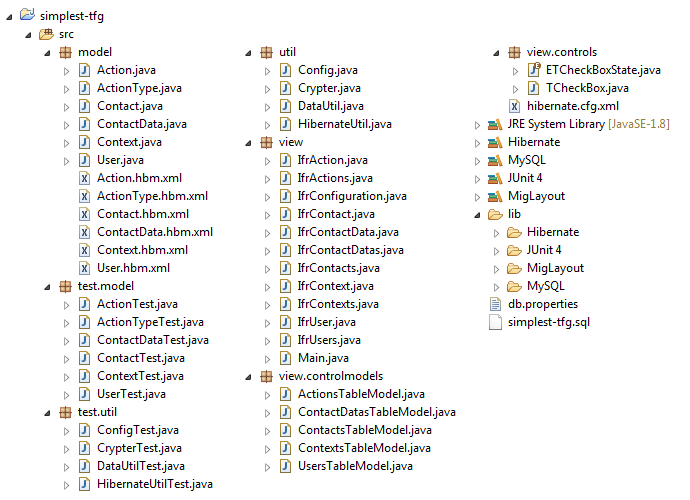
\includegraphics[scale=0.6]{stfgSrcStructure.png}
\caption{Estructura del proyecto en \program{Eclipse}}
\label{fig:stfgSrcStructure}
\end{figure}

\begin{shaded}
Debe describirse brevemente la estructura. Asimismo, se aconseja editar la imagen original para que quede similar a la del ejemplo. El motivo es porque las estructuras de carpetas suelen mostrarse de arriba a abajo, ocupando mucho espacio vertical y apenas horizontal.
\end{shaded}